\documentclass[12pt]{article}

\usepackage[a4paper,width=190mm,top=20mm,bottom=20mm,bindingoffset=6mm]{geometry}
\usepackage[utf8]{inputenc}
\usepackage[italian]{babel}
\usepackage[OT1]{fontenc}
\usepackage{graphicx}
\usepackage{float}
\usepackage{fancyhdr}
\usepackage{xcolor}
\usepackage{mathtools}
\usepackage{amsmath}
\usepackage{amssymb}
\usepackage{tikz}
\usepackage{imakeidx}
\usepackage{textcomp}
\usepackage{pifont}
\usepackage{polynom}
\usepackage{algorithm}
\usepackage{algpseudocode}
\usepackage{mathtools}
\usepackage[colorlinks=true,linkcolor=black,anchorcolor=black,filecolor=black,menucolor=black,runcolor=black,urlcolor=black]{hyperref}
\usepackage{cancel}
\usepackage{pgfplots}
\usepackage{caption}
\usepackage{tabularx}
\usepackage{comment}
\usepackage{float}
\usepackage{bm}
\usepackage{amsmath}
\usepackage{booktabs}
\usepackage{array}

\newcommand{\normsymbol}{\ensuremath{\lVert \cdot \rVert_{\text{2}}}} % Simbolo della norma 2
\newcommand{\frobnormsymbol}{\ensuremath{\lVert \cdot \rVert_{\text{F}}}} % Simbolo della norma di Frobenius


\begin{document}
    \pagestyle{fancy}
    \everymath{\displaystyle}
    \sffamily
    \begin{figure}
        \centering
        
\includegraphics[scale=0.1]{images/uniba-logo.png}
        \caption*{Università degli Studi di Bari Aldo Moro}
    \end{figure}
    
    \title{Report Progetto 1}
    \author{Emanuele Fontana}
    \date{Esame di Metodi Numerici per l'Informatica \\Anno accademico 2023/2024}
    \maketitle
    \tableofcontents\newpage
    \newpage
    \section{Introduzione}
\subsection{Traccia Progetto 1}
\begin{itemize}
    \item 

Leggere le seguenti due immagini in Matlab, usando i comandi:

\begin{verbatim}
    imt1 = imread('Bern1.bmp');
    imt2 = imread('Bern2.bmp');
    
    if(size(imt1,3)>1)
        imt1 = rgb2gray(imt1);
    end
    if(size(imt2,3)>1)
        imt2 = rgb2gray(imt2);
    end
\end{verbatim}

 \item Costruire la matrice della differenza, avendo prima trasformato i dati in tipo double:
 \begin{verbatim}
    imt1 = double(imt1)
    imt2 = double(imt2)
    Diff_Mat = abs(imt2-imt1)    
 \end{verbatim}

 
 \item Calcolare la SVD troncata di Diff
 Mat, in particolare trascrivere in Matlab almeno tre criteri
 per selezionare automaticamente il numero di componenti k da trattenere.
 \item Calcolare l’errore relativo in norma 2 e in norma di Frobenius per l’approssimazione ottenuta.
 \item Trasformare la matrice dell’approssimazione in un vettore colonna e scalare i valori tra 0 e 1.
 \item Applicare un algoritmo di binarizzazione variando la soglia (per un esempio, si veda il file
 Grad img.m).
 \item Visualizzare l’immagine finale, fancendo un opportuno “reshape” e utilizzando il comando imshow.
 L’immagine cos`ı ottenuta dovrebbe avere in bianco i pixel che identificano zone di cambiamento
 tra l’immagine I1 e l’immagine I2, mentre in nero, i pixel relativi alle zone non cambiate.
 \item Commentare i risultati

\end{itemize}

\subsection{Dati iniziali}
La matrice \textbf{Diff\_Mat} è una matrice di dimensione 301x301, in quanto le immagini \textbf{Bern1.bmp} e \textbf{Bern2.bmp} sono immagini di tale dimensione.\\
Il rank della matrice \textbf{Diff\_Mat} è 301 dunque massimo. Il che significa che tutti i valori singolari sono non nulli.\\
Le matrici U, S e V hanno dimensioni rispettivamente 301x301, 301x301 e 301x301.\\
    \newpage
    \section{Criterio 1: GUTTMAN-KEISER}

Il criterio di Guttman-Keiser per la selezione dei valori singolari da mantenere della SVD troncata prevede di mantenere i valori singolari $\sigma_i$ che sono maggiori di 1:
\begin{equation}
    \sigma_i > 1
\end{equation}
Si tratta dunque di un criterio "oggettivo" in quanto è basato su una soglia numerica ben definita.\\
In questo caso specifico tutti i valori singolari sono maggiori di 1, quindi tutti i valori singolari vengono mantenuti.\\
Il criterio in questo caso, di fatto, si è dunque rivelato inutile.


\begin{table}[H]
    \centering
    \begin{tabular}{|c|c|c|}
        \hline
        \textbf{Matrice} & \textbf{Righe} & \textbf{Colonne} \\
        \hline
        U\_troncata & 301 & 301 \\
        \hline
        S\_troncata & 301 & 301 \\
        \hline
        V\_troncata & 301 & 301 \\
        \hline
    \end{tabular}
    \caption{Dimensioni matrici troncate}
\end{table}

\begin{table}[H]
    \centering
    \begin{tabular}{|c|c|c|}
        \hline
        \textbf{Norma} & \textbf{Errore assoluto} \\
        \hline
        2 & 0.0 \\
        \hline
        Frobenius & 0.0 \\
        \hline
    \end{tabular}
    \caption{Norme ed errori}
\end{table}

\noindent Dato che tutti i valori singolari sono stati mantenuti, l'errore relativo è nullo.\\
Per la binarizzazione sono state utilizzate le seguenti soglie:
\begin{itemize}
    \item 0.25
    \item 0.5
    \item 0.75
    \item Soglia automatica calcolata con \textbf{graythresh}
\end{itemize}

\begin{figure}[H]
    \centering
     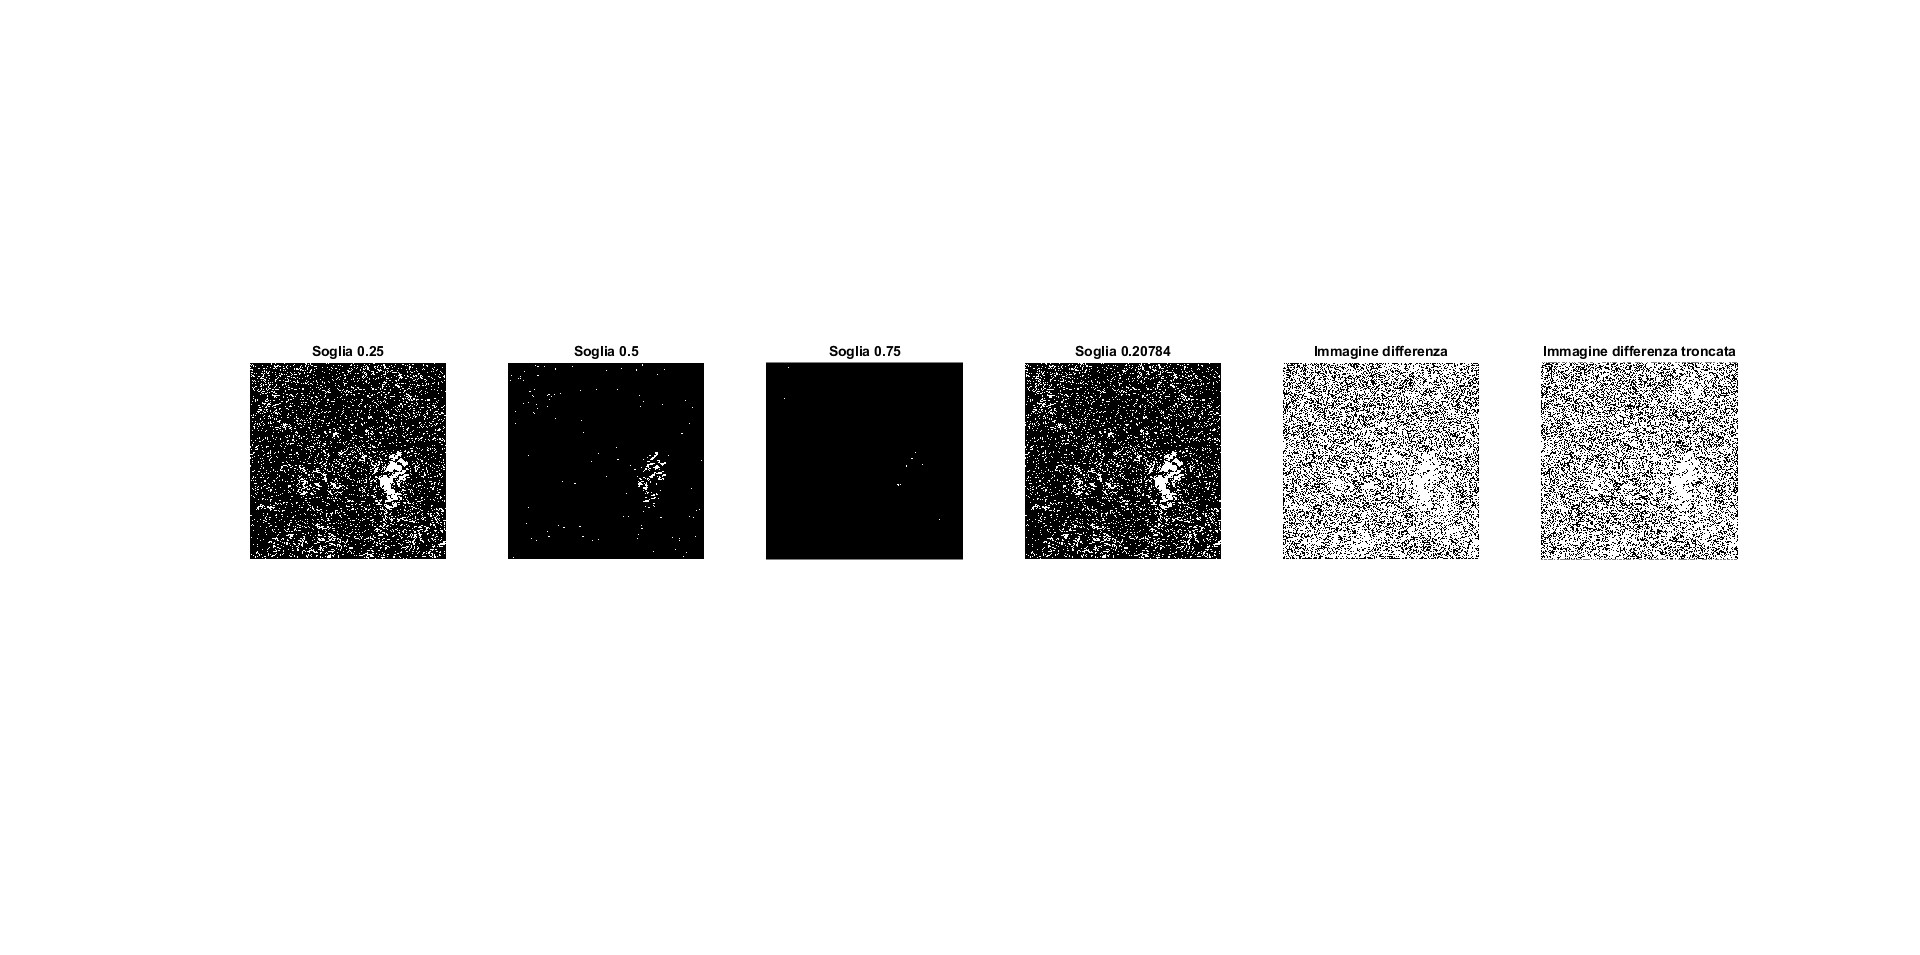
\includegraphics[width=\textwidth]{images/Criterio1.jpg}
    \caption{Immagini binarizzate con criterio 1}
\end{figure}

\noindent Come è possibile notare, ovviamente, in questo caso non vi è differenza tra l'immagine originale e quella approssimata.\\
Per quanto riguarda la binarizzazione si può notare come le soglie 0.5 e 0.75 abbiano prodootto pessimi risultati, mentre la soglia 0.25 e quella automatica abbiano prodotto risultati migliori.\\
\noindent Per il processo di troncamento sono stati necessari in media circa \textcolor{blue}{\textbf{0.0018}} secondi.\\





    \newpage
    \section{Criterio 2: SCREENPLOT DI COTTEL}

Il criterio di Screenplot di Cottel per la selezione dei valori singolari da mantenere della SVD troncata prevede di effettuare un grafico dei valori singolari $\sigma_i$ e di individuare il "gomito" del grafico e mantenere i valori singolari che si trovano prima di esso.\\

\begin{figure}[H]
    \centering
     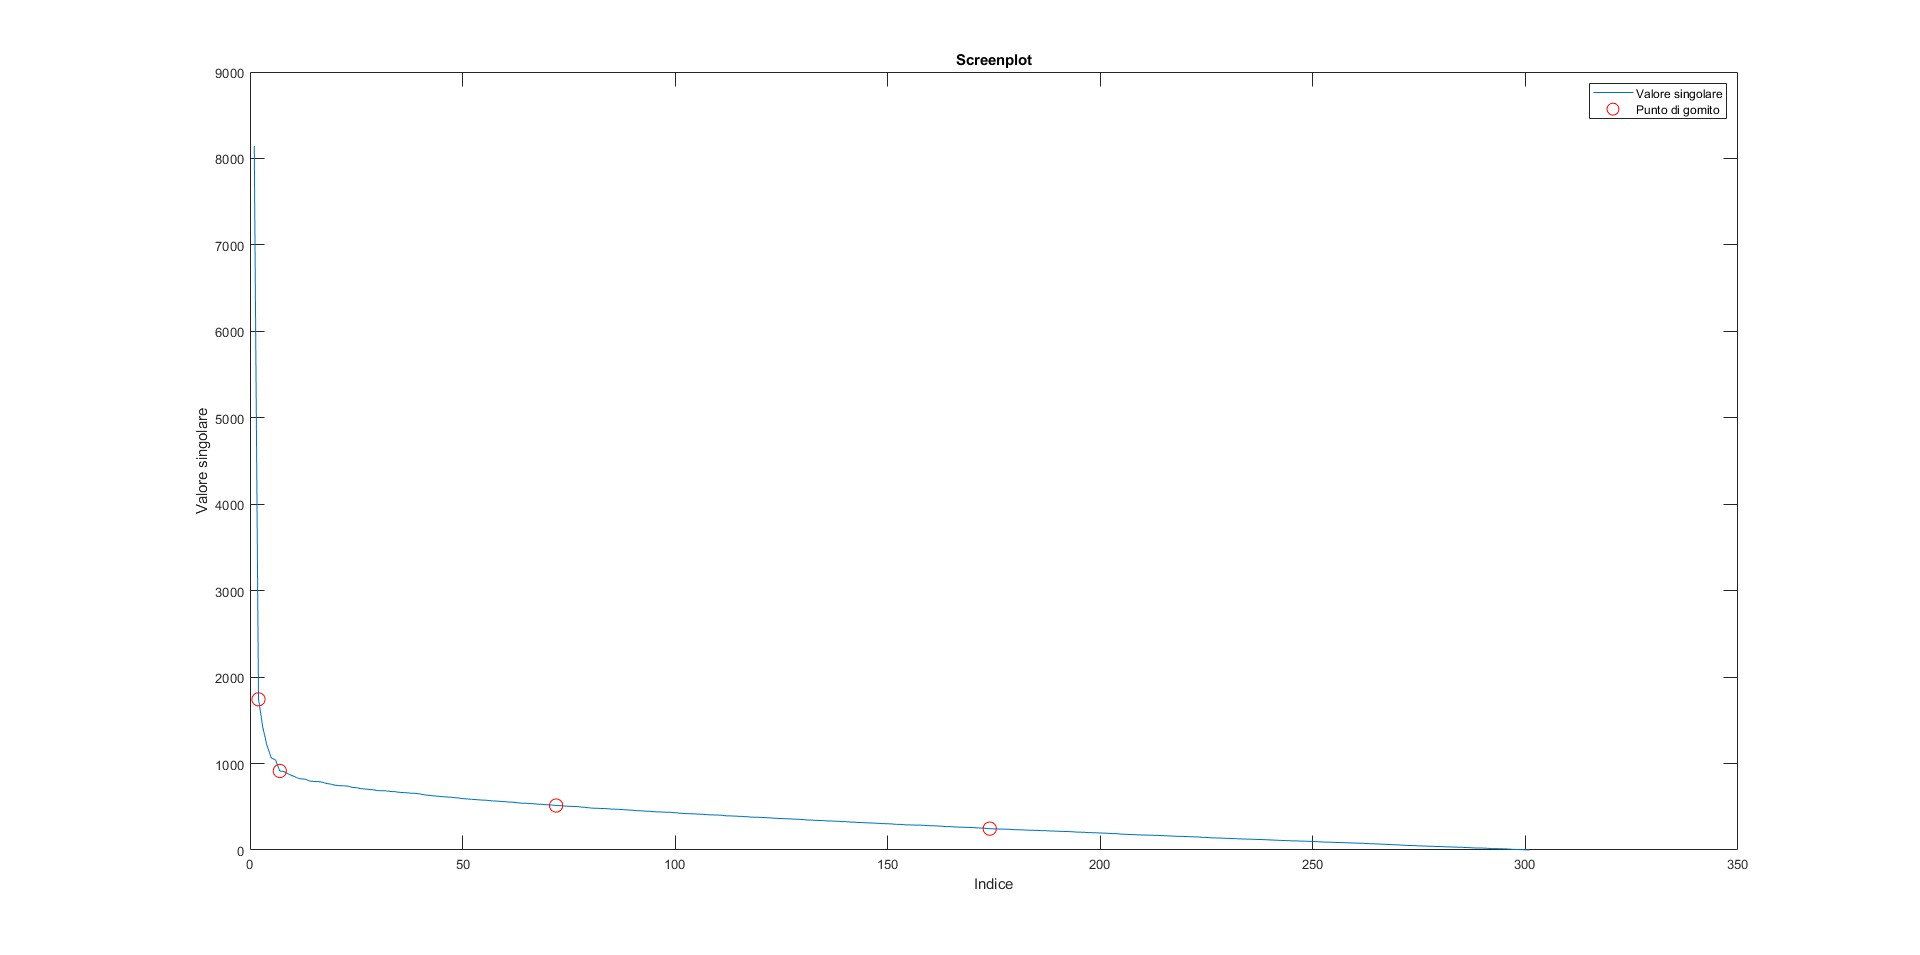
\includegraphics[width=\textwidth]{images/plot.jpg}
    \caption{Plot dei valori singolari}
\end{figure}

\noindent Mediante la funzione \textbf{findchangepts} sono stati individuati 4 punti di gomito. In questo caso si è deciso di procedere con il secondo gomito, ovvero x=7 (di fatto questo criterio è soggettivo).
Sono stati mantenuti i primi 7 valori singolari.\\
\begin{table}[H]
    \centering
    \begin{tabular}{|c|c|c|}
        \hline
        \textbf{Matrice} & \textbf{Righe} & \textbf{Colonne} \\
        \hline
        U\_troncata & 301 & 7 \\
        \hline
        S\_troncata & 7 & 7 \\
        \hline
        V\_troncata & 301 & 7 \\
        \hline
    \end{tabular}
    \caption{Dimensioni matrici troncate}
\end{table}

\begin{table}[H]
    \centering
    \begin{tabular}{|c|c|c|}
        \hline
        \textbf{Norma} & \textbf{Errore relativo} & \textbf{Errore assoluto} \\
        \hline
        2 & 0.111445 & 907.434068 \\
        \hline
        Frobenius & 0.614371 & 6782.450233 \\
        \hline
    \end{tabular}
    \caption{Norme ed errori}
\end{table}

\noindent
E' noto inoltre che l'errore assoluto in norma due risulta essere $\sigma_{k+1}$ e in norma Frobenius 
\begin{equation}
    \sqrt{\sum_{i=k+1}^{r}\sigma_i^2}
\end{equation}
 dove k è il numero di valori singolari mantenuti.\\
Per la binarizzazione sono state utilizzate le seguenti soglie:
\begin{itemize}
    \item 0.25
    \item 0.5
    \item 0.75
    \item Soglia automatica calcolata con \textbf{graythresh}
\end{itemize}

\begin{figure}[H]
    \centering
     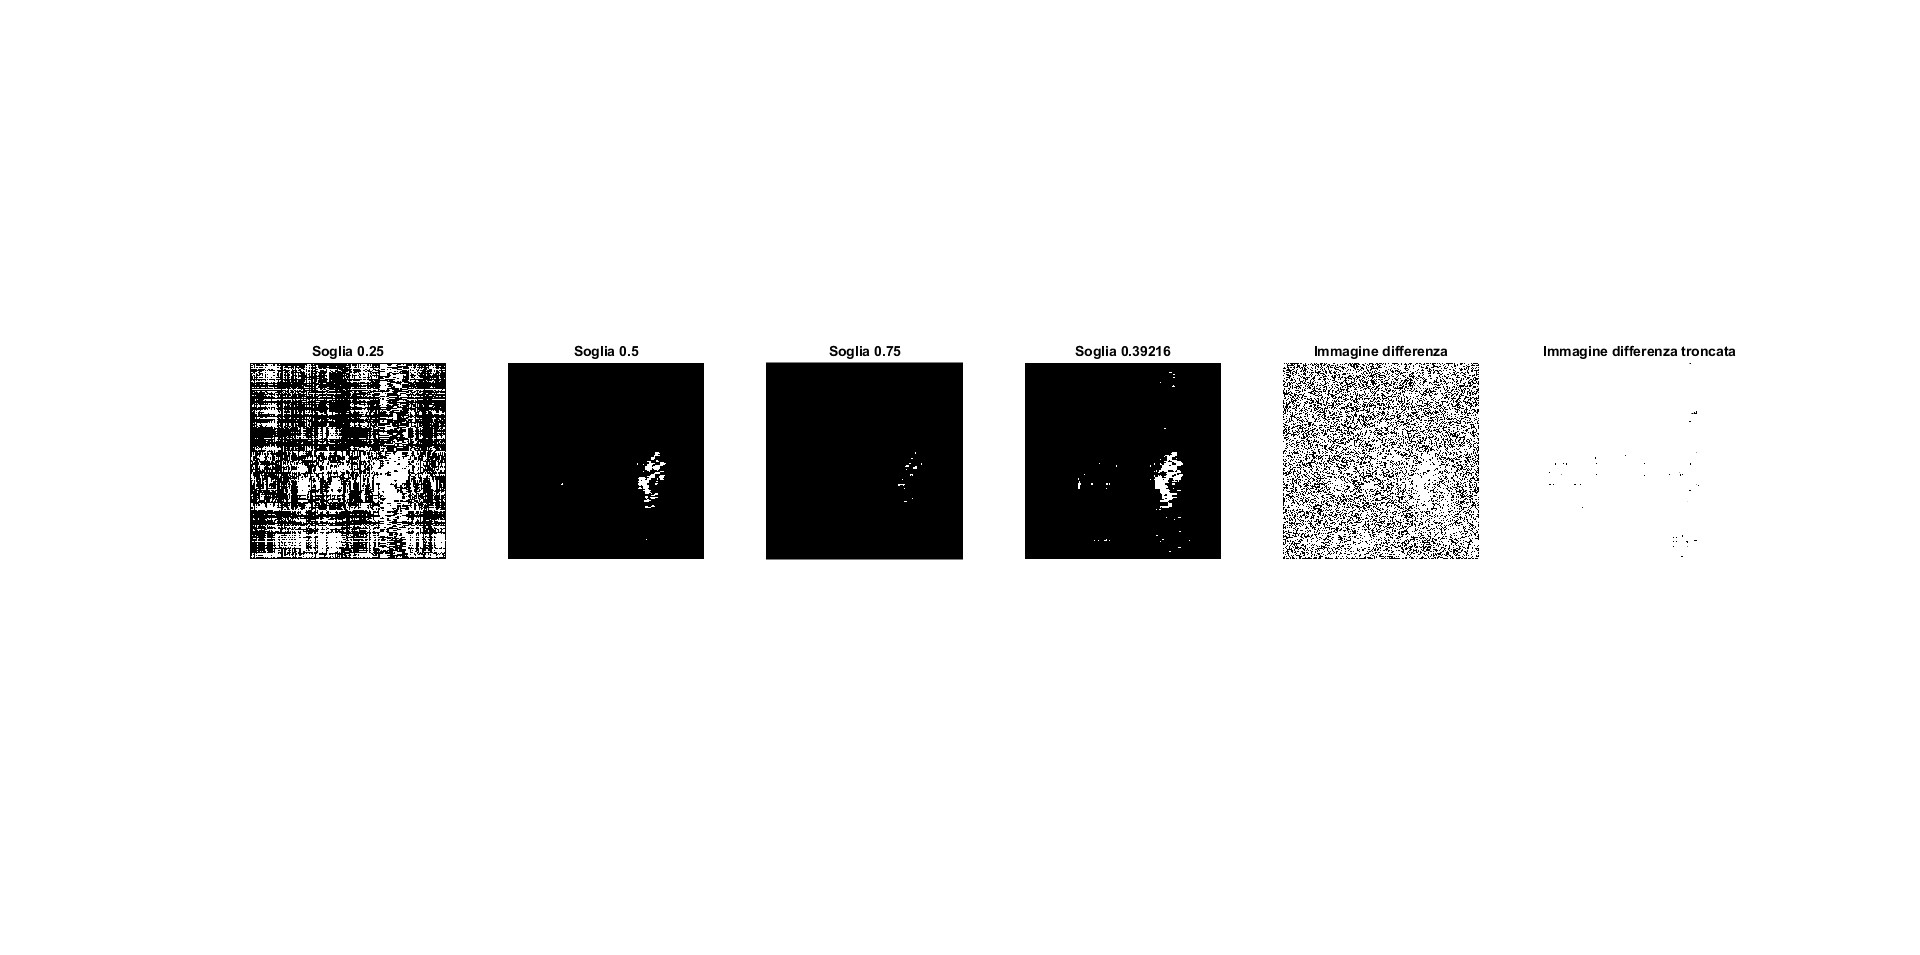
\includegraphics[width=\textwidth]{images/Criterio2.jpg}
    \caption{Immagini binarizzate con criterio 2}
\end{figure}

\noindent Come è possibile notare in questo caso vi è molta differenza tra l'immagine originale e quella approssimata.\\
Osservando le soglie di binarizzazione possiamo vedere come in questo caso la soglia automatica e la soglia 0.5 abbiano prodotto il risultato più "coerente" con l'approssimazione, mentre la soglia 0.25 ha prodotto più "coerente" con l'originale.\\

\noindent Per il processo di troncamento sono stati necessari in media circa \textcolor{blue}{\textbf{0.07}} secondi.\\




    \newpage
    \section{Criterio 3: ENTROPIA}

Il criterio basato sull'entropia prevede di calcolare il contributo di ogni valore singolare mediante la seguente formula:
\begin{equation}
    f_j=\frac{\sigma_j^2}{\sum_{i=1}^{r}\sigma_i^2}
    \label{fj:contributi}
\end{equation}
e successivamente calcolare l'entropia totale della matrice mediante la seguente formula:
\begin{equation}
    E = -\frac{1}{\log(r)}\sum_{j=1}^r f_j \log(f_j)
\end{equation}

\noindent Con questo criterio, vengono selezionati i primi $\sigma_k$ valori singolari, dove $k$ viene scelto come il più piccolo indice tale che:
\begin{equation}
\sum_{j=1}^k f_i \geq E
\end{equation}

In questo caso l'entropia totale della matrice è risultata essere 0.517648. Volendo mantenere il 75\% dell'entropia totale il k suggerito è 116.
\begin{table}[H]
    \centering
    \begin{tabular}{|c|c|c|}
        \hline
        \textbf{Matrice} & \textbf{Righe} & \textbf{Colonne} \\
        \hline
        U\_troncata & 301 & 116 \\
        \hline
        S\_troncata & 116 & 116 \\
        \hline
        V\_troncata & 301 & 116 \\
        \hline
    \end{tabular}
    \caption{Dimensioni matrici troncate}
\end{table}

\begin{table}[H]
    \centering
    \begin{tabular}{|c|c|c|}
        \hline
        \textbf{Norma} &\textbf{Errore assoluto} \\
        \hline
        2 &  384.477333 \\
        \hline
        Frobenius & 2892.327572 \\
        \hline
    \end{tabular}
    \caption{Norme ed errori}
\end{table}

\noindent
E' noto inoltre che l'errore assoluto in norma due risulta essere $\sigma_{k+1}$ e in norma Frobenius 
\begin{equation}
    \sqrt{\sum_{i=k+1}^{r}\sigma_i^2}
\end{equation}
 dove k è il numero di valori singolari mantenuti.\\
Per la binarizzazione sono state utilizzate le seguenti soglie:
\begin{itemize}
    \item 0.25
    \item 0.5
    \item 0.75
    \item Soglia automatica calcolata con \textbf{graythresh}
\end{itemize}

\begin{figure}[H]
    \centering
     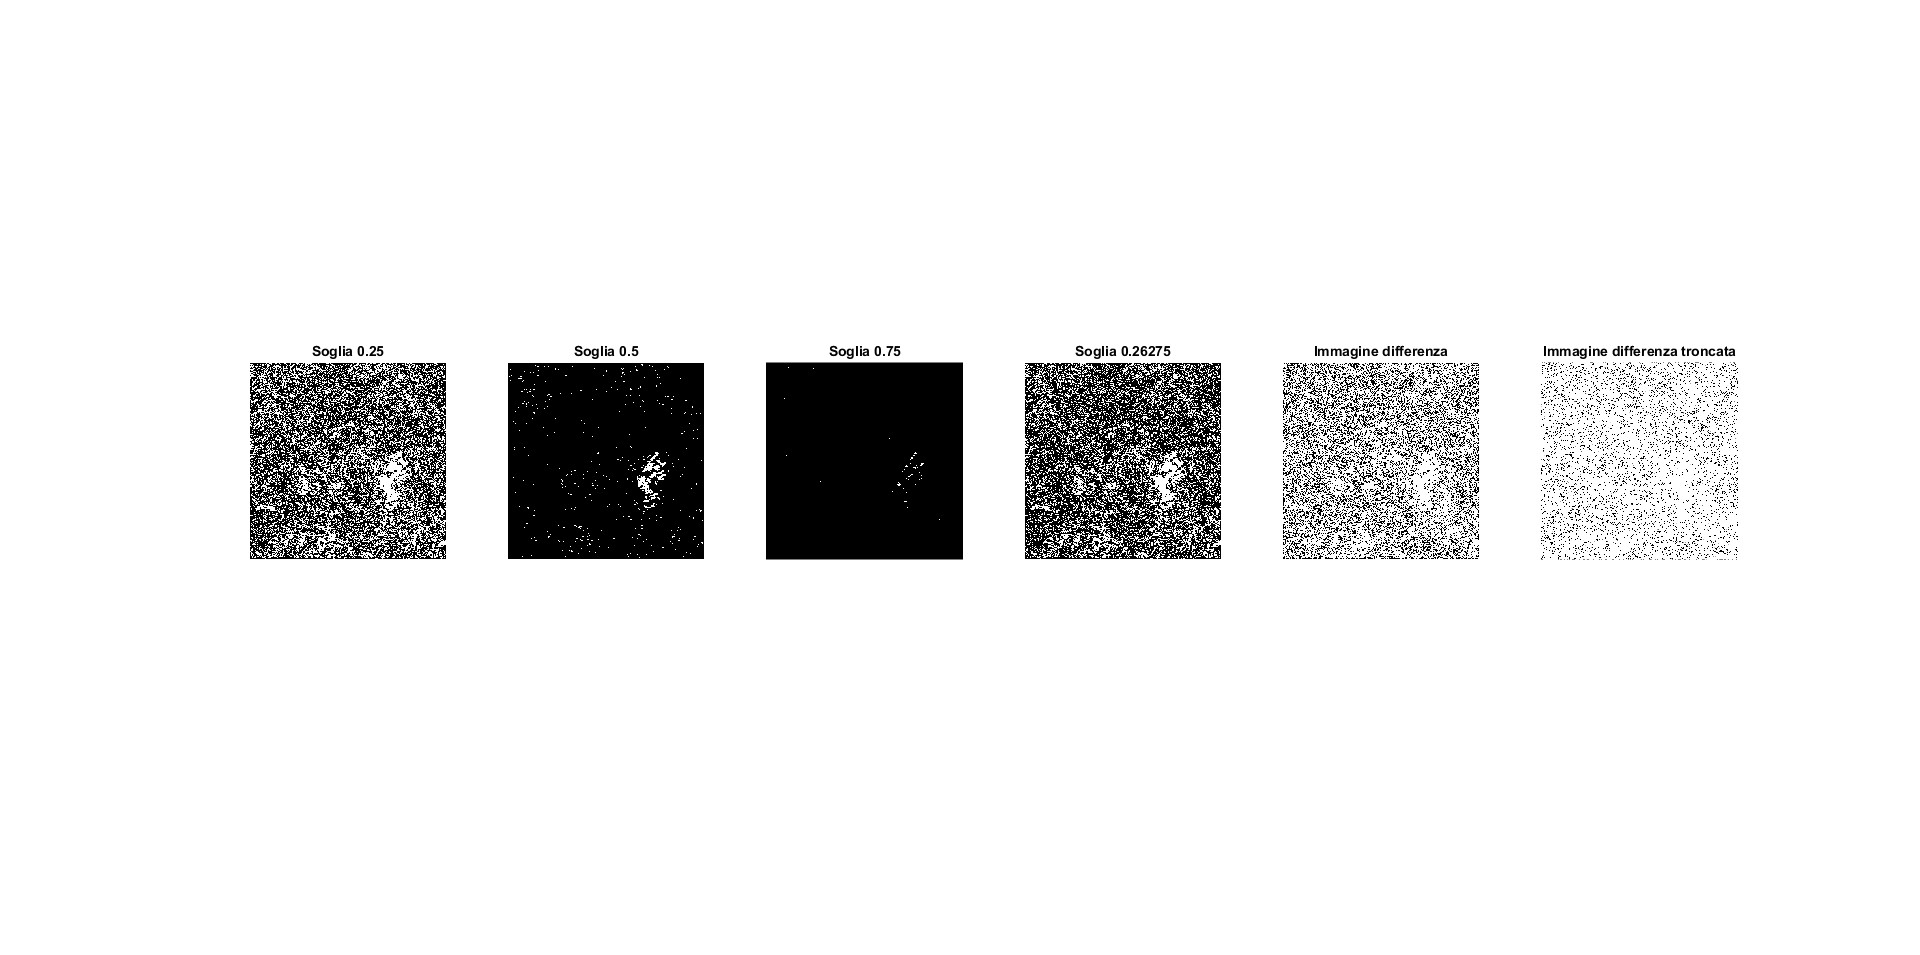
\includegraphics[width=\textwidth]{images/Criterio3.jpg}
    \caption{Immagini binarizzate con criterio 3}
\end{figure}

\noindent Le soglie 0.25 e automatica sono molto simili tra loro e sono "coerenti" sia con l'immagine originale che con quella troncata.

\noindent Per il processo di troncamento sono stati necessari in media circa \textcolor{blue}{\textbf{0.0009}} secondi.\\




    \newpage
    \section{Criterio 4: ENERGIA}

Il criterio basato sull'energia prevede di calcolare l'energia totale della matrice mediante la seguente formula:

\begin{equation}
    Energia=\sum_{j=1}^r \sigma_j^2
\end{equation}

\noindent e di scegliere un numero k di valori singolari tale che 
\begin{equation}
    \sum_{j=1}^k \sigma_j^2
\end{equation}
sia almeno il 90\% dell'energia totale.\\

\noindent In questo caso l'energia totale della matrice è risultata essere 121874051. Volendo mantenere il 90\% dell'energia totale, ovvero 109686645.9,  il k suggerito è 94, con un energia pari a 109708426.061981
\begin{table}[H]
    \centering
    \begin{tabular}{|c|c|c|}
        \hline
        \textbf{Matrice} & \textbf{Righe} & \textbf{Colonne} \\
        \hline
        U\_troncata & 301 & 94 \\
        \hline
        S\_troncata & 94 & 94 \\
        \hline
        V\_troncata & 301 & 94 \\
        \hline
    \end{tabular}
    \caption{Dimensioni matrici troncate}
\end{table}

\begin{table}[H]
    \centering
    \begin{tabular}{|c|c|c|}
        \hline
        \textbf{Norma} & \textbf{Errore relativo} & \textbf{Errore assoluto} \\
        \hline
        2 & 0.054367 & 442.680374 \\
        \hline
        Frobenius & 0.315945 & 3487.925592 \\
        \hline
    \end{tabular}
    \caption{Norme ed errori}
\end{table}

\noindent
E' noto inoltre che l'errore assoluto in norma due risulta essere $\sigma_{k+1}$ e in norma Frobenius 
\begin{equation}
    \sqrt{\sum_{i=k+1}^{r}\sigma_i^2}
\end{equation}
 dove k è il numero di valori singolari mantenuti.\\
Per la binarizzazione sono state utilizzate le seguenti soglie:
\begin{itemize}
    \item 0.25
    \item 0.5
    \item 0.75
    \item Soglia automatica calcolata con \textbf{graythresh}
\end{itemize}

\begin{figure}[H]
    \centering
     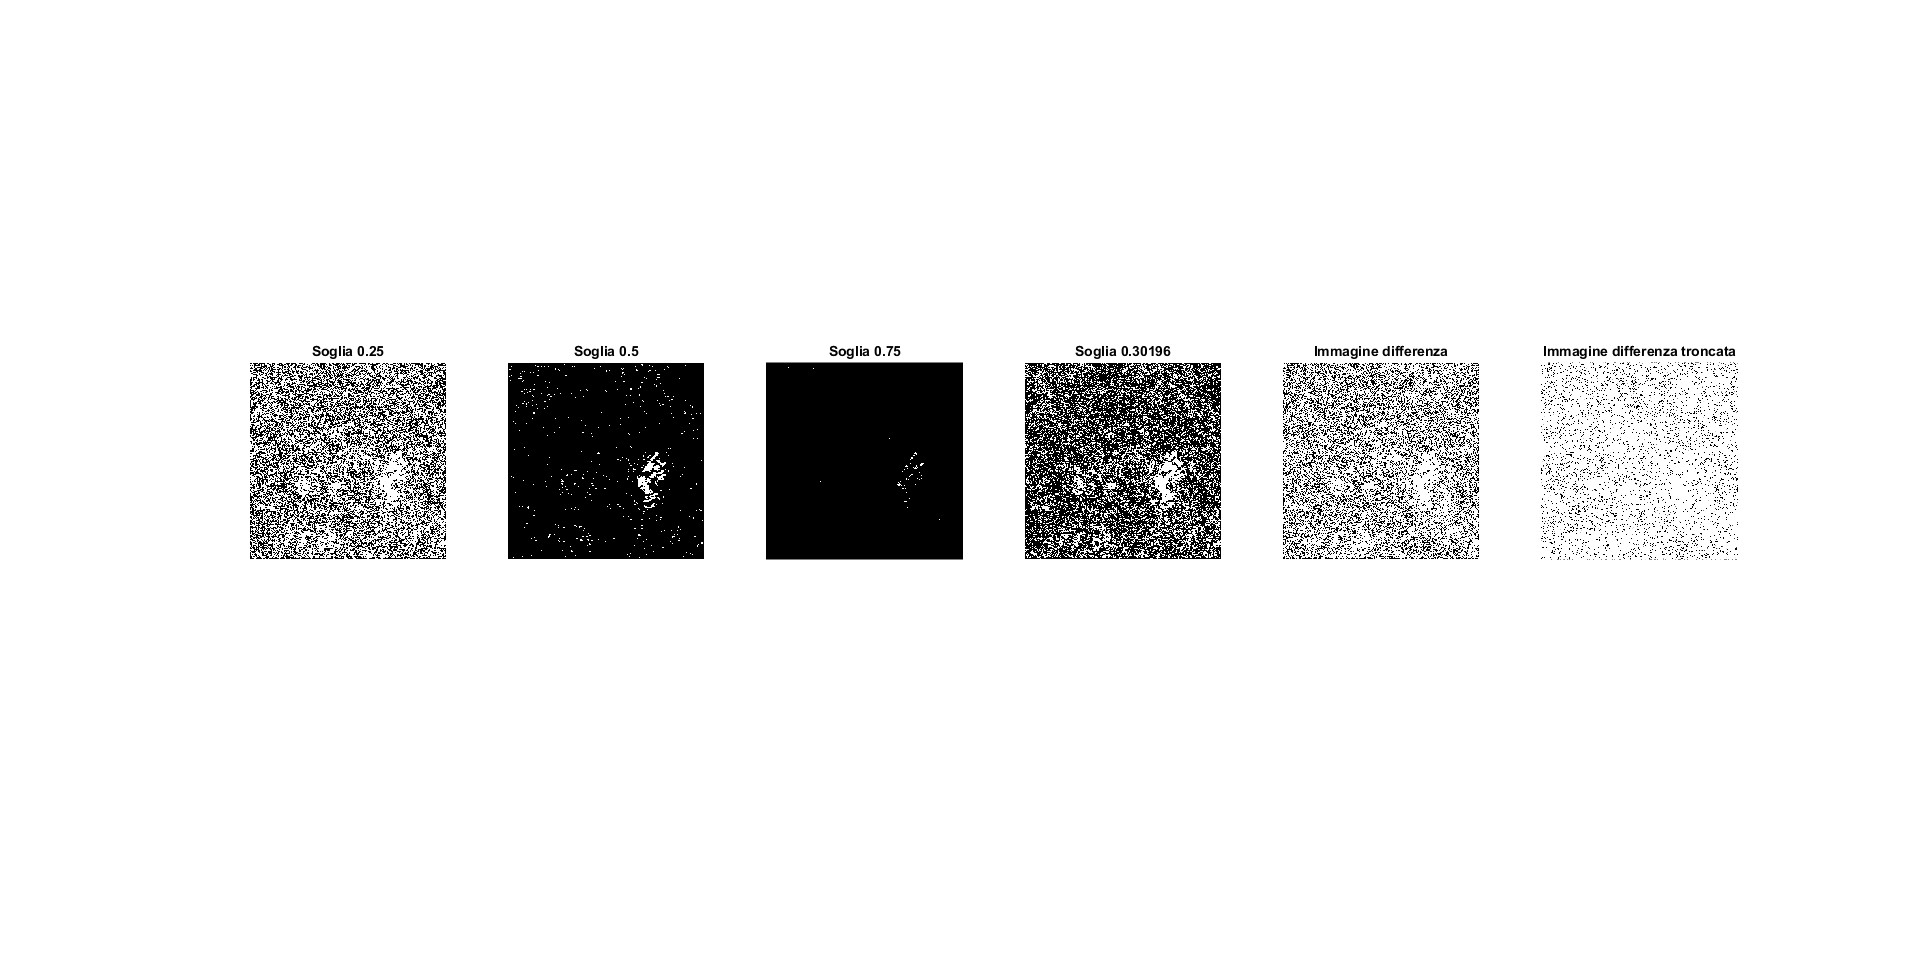
\includegraphics[width=\textwidth]{images/Criterio4.jpg}
    \caption{Immagini binarizzate con criterio 4}
\end{figure}

\noindent Le soglie 0.25 e automatica sono molto simili tra loro e sono "coerenti" sia con l'immagine originale che con quella troncata.

\noindent Per il processo di troncamento sono stati necessari in media circa \textcolor{blue}{\textbf{0.006}} secondi.\\




    \newpage
    \section{Criterio 5: K-MEANS ISOLATION FOREST}

Dati i contributi di ciascun valore singolare, descritti in (\ref{fj:contributi}), si è scelto di utilizzare il criterio K-Means Isolation Forest.\\
La prima operazione è stata quella di calcolare il logaritmo di ciascun contributo e successivamente dividere i valori in 2 cluster: \textbf{Rumore} e \textbf{Informazione}.\\
Il K-Means però è un apprendimento non supervisionato, dunque non è possibile sapere a priori quale cluster corrisponda a Rumore e quale a Informazione.\\
Poichè nei valori singolari
\begin{equation}
    \sigma_1 >= \sigma_2 >= \sigma_3 >= ... >= \sigma_r>=0
\end{equation}
allora sicuramente il cluster contenente il contributo di $\sigma_1$ sarà quello relativo all'informazione.\\
Una volta identificato tale cluster, si procede a rilevare anomalie mediante l'algoritmo di Isolation Forest.\\

\noindent Il risultato dell'algoritmo ha portato a mantere i primi 225 valori singolari
 \begin{table}[H]
    \centering
    \begin{tabular}{|c|c|c|}
        \hline
        \textbf{Matrice} & \textbf{Righe} & \textbf{Colonne} \\
        \hline
        U\_troncata & 301 & 225 \\
        \hline
        S\_troncata & 225 & 225 \\
        \hline
        V\_troncata & 301 & 225 \\
        \hline
    \end{tabular}
    \caption{Dimensioni matrici troncate}
\end{table}

\begin{table}[H]
    \centering
    \begin{tabular}{|c|c|c|}
        \hline
        \textbf{Norma} & \textbf{Errore assoluto} \\
        \hline
        2 & 141.942286  \\
        \hline
        Frobenius & 723.122392 \\
        \hline
    \end{tabular}
    \caption{Norme ed errori}
\end{table}

\noindent
E' noto inoltre che l'errore assoluto in norma due risulta essere $\sigma_{k+1}$ e in norma Frobenius 
\begin{equation}
    \sqrt{\sum_{i=k+1}^{r}\sigma_i^2}
\end{equation}
 dove k è il numero di valori singolari mantenuti.\\
Per la binarizzazione sono state utilizzate le seguenti soglie:
\begin{itemize}
    \item 0.25
    \item 0.5
    \item 0.75
    \item Soglia automatica calcolata con \textbf{graythresh}
\end{itemize}

\begin{figure}[H]
    \centering
     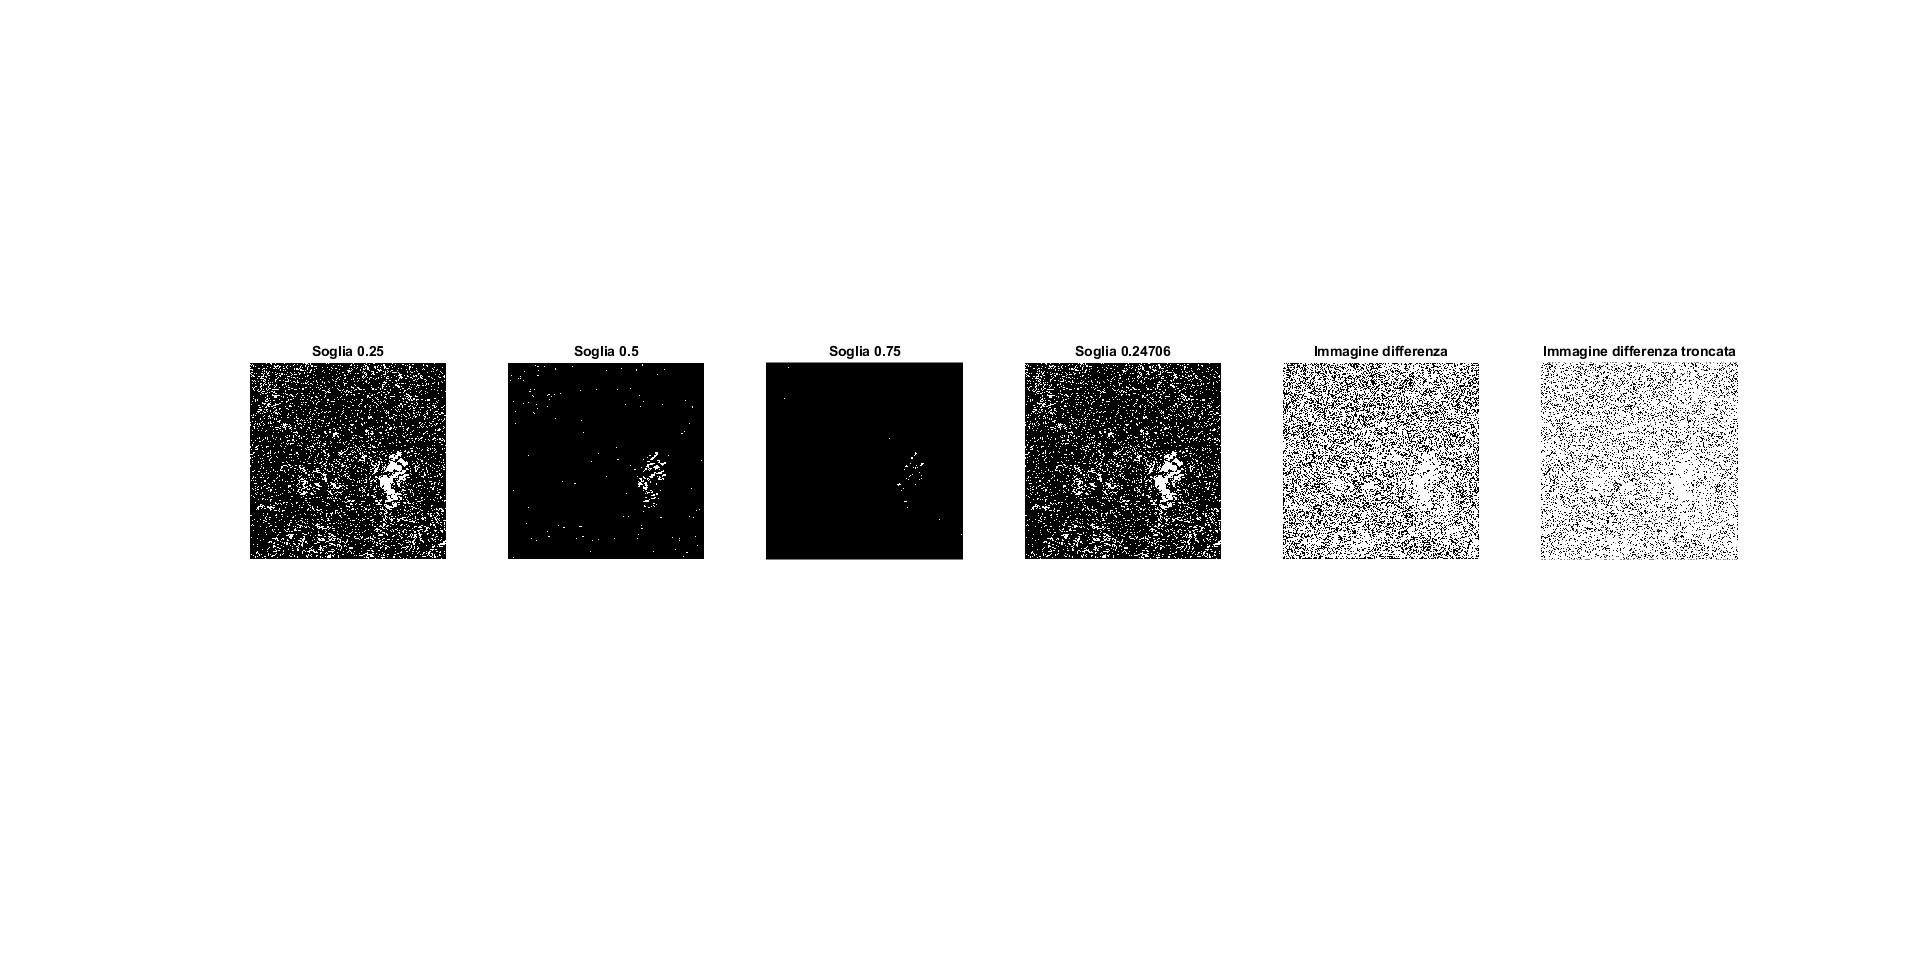
\includegraphics[width=\textwidth]{images/Criterio5.jpg}
    \caption{Immagini binarizzate con criterio 5}
\end{figure}

\noindent Le soglie 0.25 e automatica sono molto simili tra loro e sono "coerenti" sia con l'immagine originale che con quella troncata.

\noindent Per il processo di troncamento sono stati necessari in media circa \textcolor{blue}{\textbf{0.35}} secondi.\\


    \newpage
    \section{Conclusioni}

In questo progetto sono stati analizzati diversi criteri per la selezione del numero di valori singolari da mantenere nella SVD troncata di una matrice di differenza tra due immagini e diverse soglie per la binarizzazione dell'immagine risultante.\\

\begin{table}[H]
    \centering
    \resizebox{\textwidth}{!}{
    \begin{tabular}{|c|c|c|c|c|c|c|}
    \hline
     	\textbf{Criterio} & \textbf{Valore di k} & \textbf{Errore assoluto \normsymbol} & \textbf{Errore assoluto in \frobnormsymbol} & \textbf{Tempo} & \textbf{Memoria utilizzata} & \textbf{Soglia} \\
    \hline
    Guttman-Keiser & 301 & 0 & 0 & 0.0018s & 301x301 + 301 +301x301= 181.503 & 0.25 oppure 0.020784 (automatica) \\
    \hline
    Screenplot di Cottel & 7 & 907.43406 & 6782.450233 & 0.07s & 7x301 + 7 + 301x7 = 4.221 & 0.25 simile all'originale, 0.39216 (automatica) simile all'approssimazione \\
    \hline
    Entropia & 116 &  384.477333 & 2892.327572 & 0.0009s & 301x116 + 116 + 301x116 = 69.948 & 0.25 oppure 0.26275 (automatica) \\
    \hline
    Energia & 94 & 442.680374 & 3487.925592 & 0.006s & 301x94 + 94 + 301x94 = 56.682 & 0.25 oppure 0.30196 (automatica) \\
    \hline
    K-Means Isolation Forest (log) & 225 &  141.942286  & 723.122392 & 0.35s & 301x225 + 225 + 301x225 = 135.675 & 0.25 oppure 0.24706 (automatica) \\
    \hline
    K-Means Isolation Forest & 1 & 1742.857352 &  7454.849653 & 0.0055s & 301x1 + 1 + 301x1 = 603 & / \\
    \hline
    \end{tabular}
}
    \caption{Risultati}
\end{table}

\noindent Per il calcolo della memoria utilizzata si è tenuto conto delle dimensioni delle matrici U, S e V troncate, in particolare di S si tiene conto della diagonale.\\

\noindent Il criterio di Guttman-Keiser non si è rilevato utili in questo campo in quanto ha sovrastimato di molto il numero di valori singolari da mantenere, in questo caso specifico 301, che è il numero massimo possibile.\\
Il criterio di Cottel, essendo basato sullo screenplot e sulla scelta soggettiva del gomito, in questo caso ha sottostimato di molto il numero di valori singolari da mantenere, in questo caso 7.\\
Gli errori di approssimazione sono molto alti e il tempo di esecuzione è anche maggiore rispetto ad altri criteri che portano a errori minori. In questo caso una soglia più bassa scelta arbitrariamente (e non automaticamente) ha portato ad avere risultati più simili all'immagine originale che a quella troncata.\\
Il criterio del K-Means isolation forest con logaritmo è il secondo per memoria occupata e primo per tempo di esecuzione impiegato. Sono stati selezionati 225 valori singolari. Senza logaritmo risulta un metodo di fatto inutile.
Due criteri molto simili dal punto di vista di errori, tempo di esecuzione e memoria sono Entropia ed Energia. In particolare quello dell'energia ha richiesto meno tempo, occupato meno memoria al costo di un errore leggermente superiore, rivelandosi di fatto il miglior criterio.

\noindent Possiamo infine notare come in genere soglie molto basse abbiano portato a risultati migliori. In particolare la soglia 0.25 è risultata essere sempre molto simile a quella calcolata automaticamente, il che potrebbe portare vantagggi (si pensi a matrici molto più grandi in cui l'algoritmo di graythresh potrebbe impiegare molto tempo e ottenere risultati molto vicini a 0.25).\\


\end{document}
